

\begin{table}[!ht]
\centering
\resizebox{\columnwidth}{!}{\begin{tabular}{|c|c|c|c|} 
\hline
item & Machine A & Machine N & Earn profit \\
\hline
Nuts & 1 & 3  &  17.5  \\ 
\hline
Bolts & 3 & 1 &  7  \\ 
\hline
Hour's a day & 12 & 12 & \\ 
\hline
\end{tabular}}
\caption{Manufacturer produces nuts and bolts}
\label{opt/15/tab:table1}
\end{table}
Let the number of nuts  be $x$ and the number of bolts be $y$  such that 
\begin{align}
x \geq 0 \\
y \geq 0 
\end{align}
According to the question,
\begin{align}
{x} + 3{y} \leq 12
\\
3{x} + {y} \leq 12
\end{align}
$\therefore$ Our problem is
\begin{align}
\max_{\vec{x}} Z &= \myvec{17.5 & 7}\vec{x}\\
s.t. \quad \myvec{1 & 3 \\ 3 & 1}\vec{x} &\preceq \myvec{12\\12} 
\end{align}
Lagrangian function is given by
\begin{equation}
\begin{aligned}
&L(\vec{x},\boldsymbol{\lambda}) \\ &= \myvec{17.5 & 7}\vec{x}+\lcbrak{\sbrak{\myvec{1 & 3}\vec{x}-12}} \\ &+ \sbrak{\myvec{3 & 1}\vec{x}-12}\\ &+ \sbrak{\myvec{-1 & 0}\vec{x}} +\rcbrak{\sbrak{\myvec{0 & -1}\vec{x}}}\boldsymbol{\lambda}
\end{aligned}
\end{equation}
where,
\begin{align}
\boldsymbol{\lambda} &= \myvec{\lambda_1 \\ \lambda_2 \\ \lambda_3 \\ \lambda_4 \\ \lambda_5 \\ \lambda_6}
\end{align}
Now,
\begin{align}
\nabla L(\vec{x},\boldsymbol{\lambda}) &= \myvec{17.5+ \myvec{1 & 3  & -1 & 0 }\boldsymbol{\lambda}\\ 7+\myvec{3 & 1 & 0 & -1}\boldsymbol{\lambda} \\ \myvec{1 & 3}\vec{x}-12 \\ \myvec{3 & 1}\vec{x}-12 \\  \myvec{-1 & 0}\vec{x} \\ \myvec{0 & -1}\vec{x}}
\end{align}
$\therefore$ Lagrangian matrix is given by
\begin{align}
\myvec{0 & 0 & 1 & 3 & -1 & 0 \\ 0 & 0 & 3 & 1  & 0 & -1 \\ 1 & 3 & 0 & 0 & 0 & 0 \\ 3 & 1 & 0 & 0 & 0 & 0  \\ -1 & 0 & 0 & 0 & 0 & 0  \\ 0 & -1 & 0 & 0 & 0 & 0 }\myvec{\vec{x} \\ \boldsymbol{\lambda} } &= \myvec{-17.5 \\ -7 \\ 12 \\ 12 \\ 0 \\0 }
\end{align}
Considering $\lambda_1,\lambda_2$ as only active multiplier,
\begin{align}
\myvec{0 & 0 & 1 & 3 \\ 0 & 0 & 3 & 1 \\ 1 & 3 & 0 & 0 \\ 3 & 1 & 0 & 0}\myvec{\vec{x}\\ \boldsymbol{\lambda}} &= \myvec{-17.5 \\ -7 \\ 12 \\ 12}
\end{align}
resulting in,
\begin{align}
\myvec{\vec{x} \\ \boldsymbol{\lambda}} &= \myvec{0 & 0 & 1 & 3 \\ 0 & 0 & 3 & 1 \\ 1 & 3 & 0 & 0 \\ 3 & 1 & 0 & 0}^{-1}\myvec{-17.5 \\ -7 \\ 12 \\ 12}
\\
\implies   \myvec{\vec{x} \\ \boldsymbol{\lambda}} &= \myvec{0 & 0 & \frac{-1}{8} & \frac{3}{8} \\ 0 & 0 & \frac{3}{8} & \frac{-1}{8} \\ \frac{-1}{8} & \frac{3}{8} & 0 & 0 \\ \frac{3}{8} & \frac{-1}{8} & 0 & 0}\myvec{-17.5 \\ -7 \\ 12 \\ 12}
\\
\implies \myvec{\vec{x} \\ \boldsymbol{\lambda}} &= \myvec{3 \\ 3 \\ -0.5 \\ -5.7 }
\end{align}
$\because \boldsymbol{\lambda}=\myvec{-0.5 \\ -5.7} \succ \vec{0} $
\\
$\therefore$ Optimal solution is given by
\begin{align}
    \vec{x} &= \myvec{3\\3} \\
    Z &= \myvec{17.5 & 7}\vec{x} \\
    &= \myvec{17.5 & 7}\myvec{3 \\ 3} \\
    &= 73.5
\end{align}
By using cvxpy in python ,
\begin{align}
    \vec{x}=\myvec{3\\3}\\
    Z = 73.49999997
\end{align}
Hence,\boxed{x=3} Nuts and \boxed{y=3} Bolts should be used to maximum time Available profit \boxed{Z=73.5}.  This is verified in Fig. 
\ref{opt/15/fig: Graphical Solution}.	
\begin{figure}[!ht]
\centering
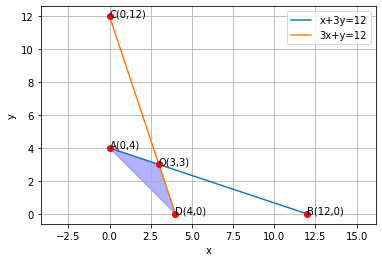
\includegraphics[width=\columnwidth]{solutions/su2021/2/15/download (2).png}
\caption{Graphical Solution}
\label{opt/15/fig: Graphical Solution}	
\end{figure}
